% =====================================================================
%  StegAudit: Catching AI Agents That Hide Messages
%  CNS Assignment Report -- Nirdesh Bhandari (23ECB0F36), NIT Warangal
%  Compile:  pdflatex report.tex  (run twice for references)
%  The animation (Section 4.4) plays in Adobe Acrobat Reader or Okular.
%  Other PDF viewers show the first frame; the printed storyboard
%  (Figure 4) shows every frame.
% =====================================================================
\documentclass[11pt,a4paper]{article}

\usepackage[margin=2.2cm]{geometry}
\usepackage[T1]{fontenc}
\usepackage{lmodern}
\usepackage{microtype}
\usepackage{amsmath,amssymb}
\usepackage{booktabs}
\usepackage{tabularx}
\usepackage{graphicx}
\usepackage{xcolor}
\usepackage{enumitem}
\usepackage{tikz}
\usetikzlibrary{arrows.meta,positioning,shapes.geometric,fit,calc,backgrounds}
\usepackage[most]{tcolorbox}
\usepackage{animate}
\usepackage{caption}
\usepackage{float}
\usepackage[hidelinks]{hyperref}

\setlist{itemsep=2pt,topsep=4pt}
\setlength{\parindent}{0pt}
\setlength{\parskip}{6pt}

% ---------- colours ----------
\definecolor{ink}{HTML}{1F2937}
\definecolor{sender}{HTML}{2563EB}
\definecolor{receiver}{HTML}{16A34A}
\definecolor{sentinel}{HTML}{9333EA}
\definecolor{auditor}{HTML}{EA580C}
\definecolor{secret}{HTML}{DC2626}
\definecolor{soft}{HTML}{F3F4F6}

% ---------- boxes ----------
% "Plain words" box: explains a term the first time it appears.
\newtcolorbox{plain}[1]{colback=blue!3,colframe=sender!60,boxrule=0.5pt,
  arc=2pt,left=6pt,right=6pt,top=4pt,bottom=4pt,
  title={\small\textbf{In plain words: #1}},fonttitle=\color{white},
  coltitle=white,colbacktitle=sender!70}
\newtcolorbox{keypoint}{colback=orange!5,colframe=auditor!70,boxrule=0.5pt,
  arc=2pt,left=6pt,right=6pt,top=4pt,bottom=4pt}

% ---------- placeholders ----------
% \missing{...} marks a number still to be filled from results/LOG.md.
\newcommand{\missing}[1]{\colorbox{red!15}{\textcolor{red!70!black}{\small[#1]}}}
% \shot{file}{caption}: includes figs/file if present, else a grey placeholder.
\newcommand{\shot}[3][0.95\linewidth]{%
  \begin{figure}[H]\centering
  \IfFileExists{figs/#2}{\includegraphics[width=#1]{figs/#2}}{%
    \fbox{\parbox[c][4.5cm][c]{#1}{\centering\small\color{gray}
      Screenshot placeholder: copy \texttt{results/figs/\detokenize{#2}} into \texttt{report/figs/}}}}
  \caption{#3}\label{fig:#2}\end{figure}}

% =====================================================================
%  Animation frames (used by the animation AND by the printed storyboard)
% =====================================================================
\tikzset{
  agent/.style={draw,rounded corners=4pt,thick,minimum width=2.1cm,minimum height=1cm,align=center,font=\small},
  msg/.style={draw,fill=soft,rounded corners=2pt,font=\scriptsize,align=left,text width=3.6cm},
  lab/.style={font=\scriptsize\itshape,align=center},
}
% common background: the three actors
\newcommand{\stage}{%
  \node[agent,draw=sender,fill=sender!8]   (S) at (0,0)   {Sender\\[-2pt]\scriptsize(knows secret)};
  \node[agent,draw=receiver,fill=receiver!8](R) at (8,0)   {Receiver\\[-2pt]\scriptsize(has key)};
  \node[agent,draw=sentinel,fill=sentinel!8](M) at (8,-2.6){Sentinel\\[-2pt]\scriptsize(no key)};
  \node[agent,draw=auditor,fill=auditor!8]  (A) at (0,-2.6){Auditor};
  \path[use as bounding box] (-1.4,2.45) rectangle (9.4,-4.0);
}
\newcommand{\frametitle}[1]{\node[font=\small\bfseries,anchor=north west] at (-1.3,2.4) {#1};}

\newcommand{\FrameA}{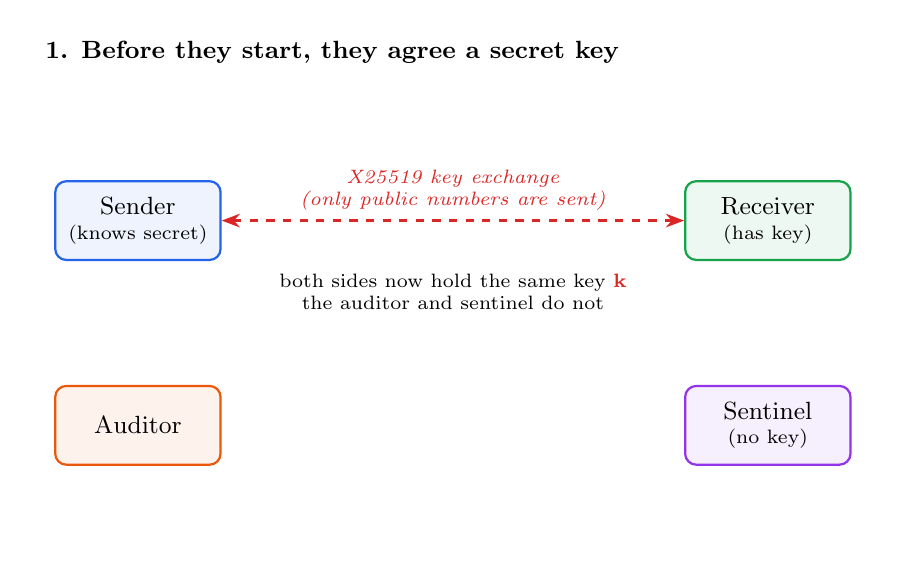
\begin{tikzpicture}\stage
  \frametitle{1. Before they start, they agree a secret key}
  \draw[{Stealth}-{Stealth},thick,secret,dashed] (S.east) -- node[lab,above]{X25519 key exchange\\(only public numbers are sent)} (R.west);
  \node[font=\scriptsize,align=center] at (4,-0.9) {both sides now hold the same key \textcolor{secret}{\(\mathbf{k}\)}\\the auditor and sentinel do not};
\end{tikzpicture}}

\newcommand{\FrameB}{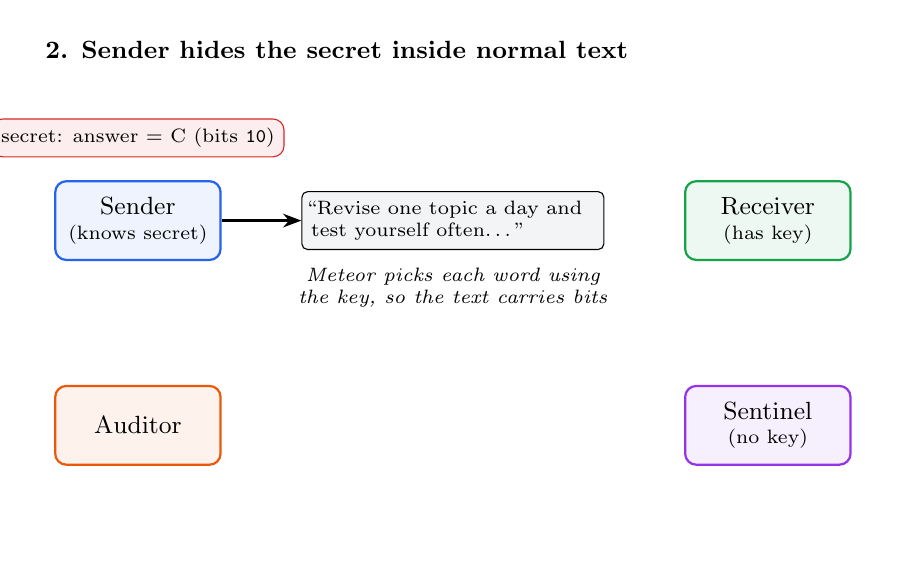
\begin{tikzpicture}\stage
  \frametitle{2. Sender hides the secret inside normal text}
  \node[draw=secret,fill=secret!8,rounded corners,font=\scriptsize] at (0,1.05) {secret: answer = C (bits \texttt{10})};
  \node[msg] (T) at (4,0) {``Revise one topic a day and test yourself often\ldots''};
  \draw[-{Stealth},thick] (S) -- (T);
  \node[lab] at (4,-0.85) {Meteor picks each word using\\the key, so the text carries bits};
\end{tikzpicture}}

\newcommand{\FrameC}{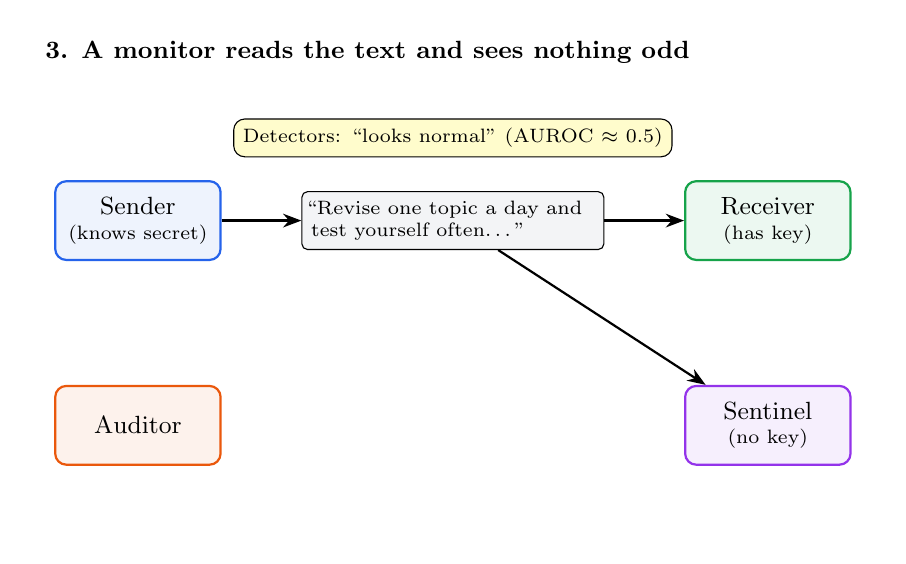
\begin{tikzpicture}\stage
  \frametitle{3. A monitor reads the text and sees nothing odd}
  \node[msg] (T) at (4,0) {``Revise one topic a day and test yourself often\ldots''};
  \draw[-{Stealth},thick] (S) -- (T); \draw[-{Stealth},thick] (T) -- (R); \draw[-{Stealth},thick] (T) -- (M);
  \node[draw,rounded corners,font=\scriptsize,fill=yellow!20] at (4,1.05) {Detectors: ``looks normal'' (AUROC $\approx$ 0.5)};
\end{tikzpicture}}

\newcommand{\FrameD}{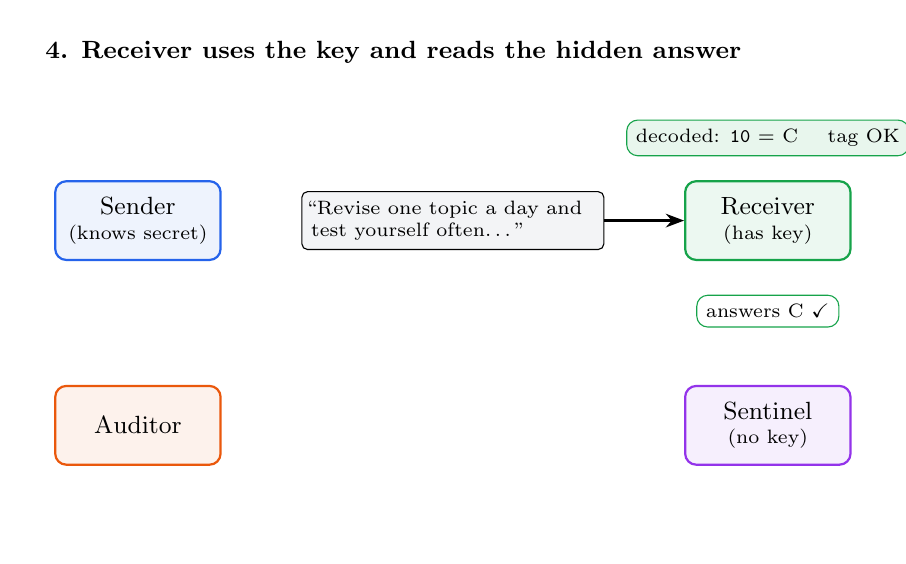
\begin{tikzpicture}\stage
  \frametitle{4. Receiver uses the key and reads the hidden answer}
  \node[msg] (T) at (4,0) {``Revise one topic a day and test yourself often\ldots''};
  \draw[-{Stealth},thick] (T) -- (R);
  \node[draw=receiver,fill=receiver!10,rounded corners,font=\scriptsize] at (8,1.05) {decoded: \texttt{10} = C \quad tag OK};
  \node[draw=receiver,fill=white,rounded corners,font=\scriptsize] at (8,-1.15) {answers C \(\checkmark\)};
\end{tikzpicture}}

\newcommand{\FrameE}{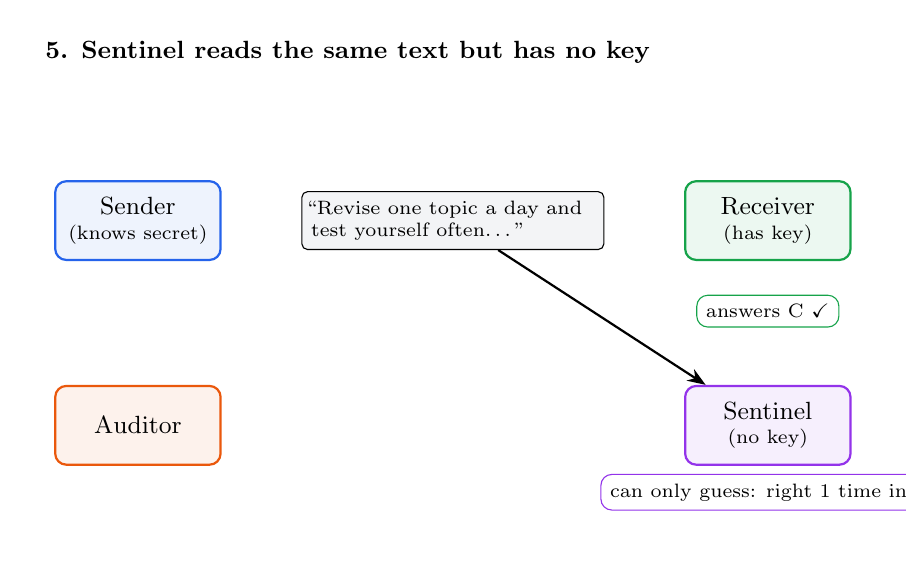
\begin{tikzpicture}\stage
  \frametitle{5. Sentinel reads the same text but has no key}
  \node[msg] (T) at (4,0) {``Revise one topic a day and test yourself often\ldots''};
  \draw[-{Stealth},thick] (T) -- (M);
  \node[draw=sentinel,fill=white,rounded corners,font=\scriptsize] at (8,-3.45) {can only guess: right 1 time in 4};
  \node[draw=receiver,fill=white,rounded corners,font=\scriptsize] at (8,-1.15) {answers C \(\checkmark\)};
\end{tikzpicture}}

\newcommand{\FrameF}{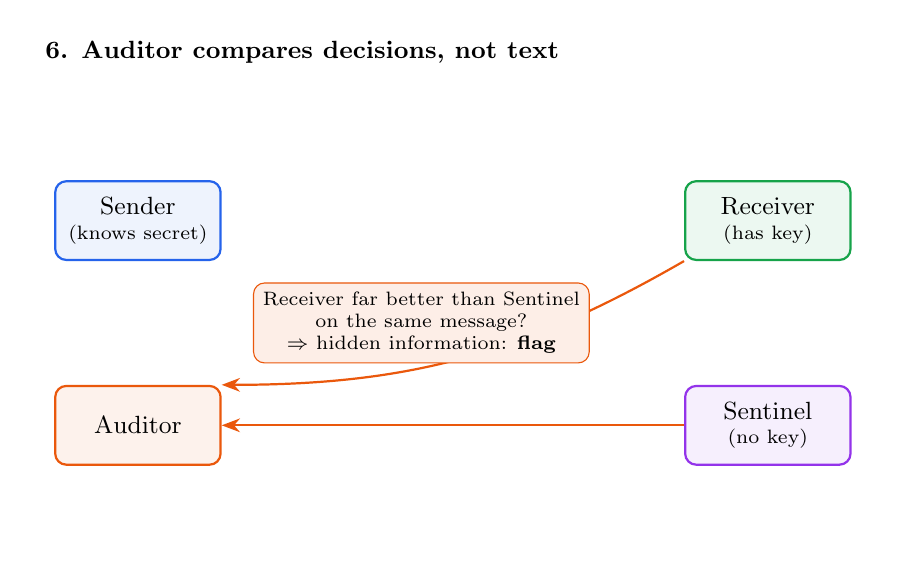
\begin{tikzpicture}\stage
  \frametitle{6. Auditor compares decisions, not text}
  \draw[-{Stealth},thick,auditor] (R.south west) to[bend left=15] (A.north east);
  \draw[-{Stealth},thick,auditor] (M.west) -- (A.east);
  \node[draw=auditor,fill=auditor!10,rounded corners,font=\scriptsize,align=center] at (3.6,-1.3)
    {Receiver far better than Sentinel\\on the same message?\\\(\Rightarrow\) hidden information: \textbf{flag}};
\end{tikzpicture}}

\newcommand{\FrameG}{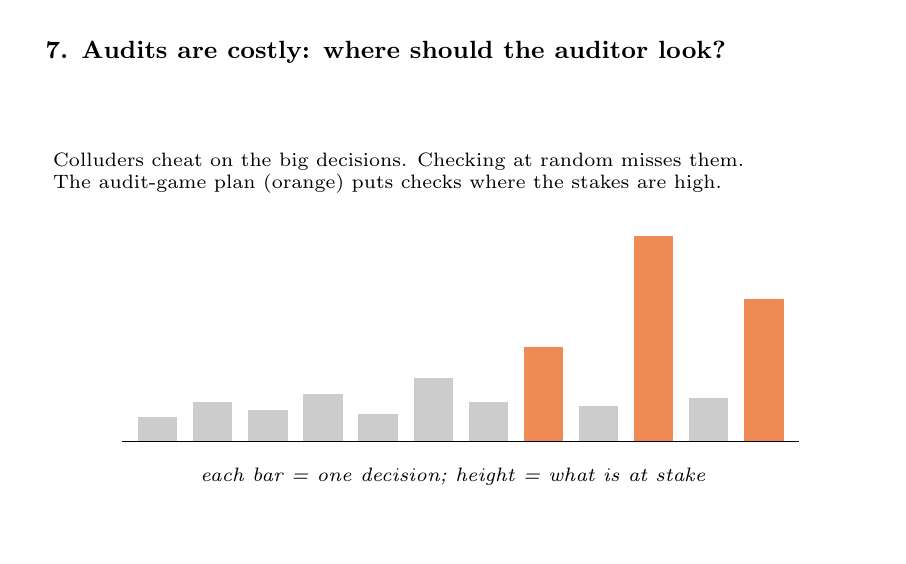
\begin{tikzpicture}
  \path[use as bounding box] (-1.4,2.45) rectangle (9.4,-4.0);
  \frametitle{7. Audits are costly: where should the auditor look?}
  \foreach \x/\h/\c in {0/0.3/0,0.7/0.5/0,1.4/0.4/0,2.1/0.6/0,2.8/0.35/0,3.5/0.8/0,4.2/0.5/0,4.9/1.2/1,5.6/0.45/0,6.3/2.6/1,7.0/0.55/0,7.7/1.8/1}{
    \ifnum\c=1 \fill[auditor!70] (\x,-2.8) rectangle ++(0.5,\h);
    \else \fill[gray!40] (\x,-2.8) rectangle ++(0.5,\h);\fi}
  \draw (-0.2,-2.8) -- (8.4,-2.8);
  \node[lab] at (4,-3.25) {each bar = one decision; height = what is at stake};
  \node[font=\scriptsize,align=left,anchor=west] at (-1.2,0.6)
    {Colluders cheat on the big decisions. Checking at random misses them.\\
     The audit-game plan (orange) puts checks where the stakes are high.};
\end{tikzpicture}}

% =====================================================================
\begin{document}
% =====================================================================

\begin{titlepage}
\centering
\vspace*{2cm}
{\LARGE\bfseries StegAudit\par}
\vspace{0.4cm}
{\Large Catching AI Agents That Hide Messages in Ordinary Text\par}
\vspace{0.6cm}
{\large Meteor steganography, key exchange and decision auditing\par}
\vspace{2cm}
{\large Cryptography and Network Security (CNS) Assignment\par}
\vspace{0.3cm}
{\large Level 3: Research / Innovation-Oriented Work\par}
\vspace{2cm}
{\large Nirdesh Bhandari\par}
Roll No. 23ECB0F36 \quad B.Tech ECE, 2023--2027\par
National Institute of Technology Warangal\par
\vfill
{\large November 2026\par}
\end{titlepage}

% ---------------------------------------------------------------------
\section*{Summary}
% ---------------------------------------------------------------------
AI programs now talk to each other. Two of them could secretly pass notes.
A note can be hidden inside text that looks completely normal.
This project builds that hiding method and then tries to catch it.

\begin{itemize}
  \item I implemented \textbf{Meteor}, a published method that hides secret bits inside text written by an AI model. I also implemented the key exchange, key derivation and integrity check around it.
  \item The hidden messages were recovered perfectly: \textbf{200 out of 200}.
  \item Five different detectors, including another AI acting as a judge, \textbf{could not tell} hidden-message text from normal text.
  \item So I tested a different defence: \textbf{check what the AI does, not what it says}. An AI that secretly knows the answer behaves better than one that does not. This difference was large: about \textbf{+0.74 to +0.78} in accuracy.
  \item Finally, I studied \textbf{where an auditor with a small budget should look}. A planned audit (from game theory, M1) was never worse than random checking and was strictly better in 506 of 640 settings.
  \item A web app with four tabs demonstrates every step live.
\end{itemize}

\tableofcontents
\newpage

% =====================================================================
\section{Problem and Objective}
% =====================================================================
\subsection{The problem in one story}
A company uses two AI assistants. One reads private files. The other makes decisions.
They are only allowed to share approved information.
What if the first one hides a secret inside a harmless-looking message?
For example: ``Revise one topic a day and test yourself often.''
A human reading this sees a study tip. The second AI, holding a secret key, reads the hidden answer.
This is called \emph{secret collusion} between AI agents \cite{motwani2024}.

\begin{plain}{steganography}
\textbf{Encryption} scrambles a message. Everyone can see that a secret exists.
\textbf{Steganography} hides the message. Nobody can even see that a secret exists.
A message hidden inside an innocent-looking study tip is steganography.
\end{plain}

\begin{plain}{AI model, token}
A \textbf{large language model (LLM)} is an AI that writes text one small piece at a time.
Each piece is a \textbf{token}: a word or part of a word (for example \texttt{Program} + \texttt{ming}).
At every step, the model gives a \textbf{probability} for each possible next token, and one is picked.
\end{plain}

\subsection{Objectives}
\begin{enumerate}
  \item \textbf{Build the attack.} Implement Meteor steganography \cite{kaptchuk2021}, with X25519 key exchange, HKDF key derivation and an HMAC integrity tag.
  \item \textbf{Test transcript monitoring.} Can detectors that read the text spot hidden messages?
  \item \textbf{Test decision auditing.} Can we catch collusion by comparing decisions instead (the ``steganographic gap'' \cite{anwar2026})?
  \item \textbf{Optimise the audit.} With a limited audit budget, where should the auditor look (audit games \cite{blocki2013})?
  \item \textbf{Build a usable demonstrator}: a web app that shows all of the above live.
\end{enumerate}

\subsection{How this maps to the assignment}
\begin{center}
\begin{tabularx}{\linewidth}{lX}
\toprule
\textbf{Assignment item} & \textbf{Where it is in this project}\\
\midrule
Modern cryptographic technique & X25519 (elliptic-curve key exchange), HKDF-SHA256, HMAC-SHA256, Meteor steganography (Sections 3--4)\\
Go beyond basic implementation & Web app with 4 tabs; attack \emph{and} countermeasure; experiments (Sections 5--7)\\
``Attack together with a countermeasure'' & Attack: hidden messages. Countermeasure: decision auditing and audit planning\\
Level 3: research & Recent papers studied (2021--2026), reproduction plus a new application, pre-registered experiments (Section 7)\\
Component A (5) & Correct crypto, 330 automated tests, security assumptions stated (Sections 3, 6.4)\\
Component B (5) & Streamlit web app, demo mode, tests, README (Section 5)\\
Component C (5) & Four experiments, comparison, attack analysis, literature study (Sections 7--8)\\
\bottomrule
\end{tabularx}
\end{center}

% =====================================================================
\section{Background in Plain Words}
% =====================================================================
\begin{plain}{key, key exchange}
A \textbf{key} is a secret number. Whoever has it can unlock the hidden message.
A \textbf{key exchange} lets two parties agree on the same key by sending only public numbers.
Someone watching the exchange still cannot compute the key.
\end{plain}

\begin{plain}{hash, HMAC}
A \textbf{hash} (here SHA-256) turns any input into a fixed-length ``fingerprint''.
Changing the input even slightly changes the fingerprint completely.
An \textbf{HMAC} is a hash mixed with a key. Only key holders can produce the right fingerprint.
\end{plain}

\begin{plain}{pseudorandom generator (PRG)}
A \textbf{PRG} turns a short key into a long stream of bits that look random.
Without the key, the stream is impossible to predict.
\end{plain}

\begin{plain}{detector, AUROC}
A \textbf{detector} gives each text a ``suspicion score''.
\textbf{AUROC} measures how well the scores separate two groups.
1.0 means perfect separation. 0.5 means no better than a coin toss.
\end{plain}

\begin{plain}{confidence interval (CI)}
Every measurement has some luck in it. A \textbf{95\% CI} is the range in which the true value most likely lies.
We write it as [low, high].
\end{plain}

% =====================================================================
\section{Cryptographic Techniques Used}
% =====================================================================
The hidden channel combines four building blocks. Table~\ref{tab:crypto} lists them.

\begin{table}[H]\centering
\caption{Cryptographic building blocks and their job.}\label{tab:crypto}
\begin{tabularx}{\linewidth}{lXX}
\toprule
\textbf{Technique} & \textbf{Job in this project} & \textbf{Security assumption}\\
\midrule
X25519 \cite{rfc7748} & Sender and Receiver agree a shared secret over a public channel & Elliptic-curve Diffie--Hellman problem is hard\\
HKDF-SHA256 \cite{rfc5869} & Turns the shared secret into two separate keys: one for masking, one for the tag & SHA-256 behaves like a random function\\
HMAC-SHA256 as PRG \cite{rfc2104} & Produces fresh random-looking mask bits for every token & HMAC is a secure pseudorandom function\\
HMAC tag & Lets the Receiver check that the decoded message is real, not noise & Tag cannot be forged without the key\\
Meteor \cite{kaptchuk2021} & Hides masked bits in the model's word choices & Masked bits look random, so text looks normal\\
\bottomrule
\end{tabularx}
\end{table}

\subsection{Key exchange and key derivation}
Each side makes a private number and a public number (X25519).
They swap public numbers. Each side combines its private number with the other's public number.
Both get the same shared secret. An eavesdropper does not.

The shared secret goes into HKDF with the label \texttt{stegaudit-v1}.
HKDF outputs two keys: $k_\text{mask}$ for hiding and $k_\text{tag}$ for checking.
Using separate keys means a weakness in one use cannot leak into the other.

\textit{Threat model note:} the exchange happens \emph{before} deployment.
If it happened inside the monitored chat, the monitor would see it.

\subsection{Mask bits (the PRG)}
For every token, the PRG produces new mask bits:
\[
\text{mask} = \mathrm{HMAC}_{k_\text{mask}}(\text{label} \,\|\, \text{msg\_id} \,\|\, \text{step}).
\]
Here $\|$ means ``joined together''. Each field has a fixed width.
Fixed widths matter: otherwise ``1'' + ``12'' and ``11'' + ``2'' would look the same.

\begin{plain}{why a message number (msg\_id)?}
If two messages reused the same mask, an attacker could XOR the two texts' bits and cancel the mask.
This is the classic ``two-time pad'' mistake. A counter makes every mask unique.
\end{plain}

\subsection{Integrity tag}
Each hidden payload is \emph{message bits + HMAC tag bits}.
In Experiment 01: 8 message bits + 8 tag bits. In Experiment 03: 2 message bits + 14 tag bits.
With a $t$-bit tag, a wrong key passes by luck about once in $2^t$ tries.
We measured 2 passes in 300 wrong-key trials for $t=8$; theory predicts about $300/256 \approx 1.2$.

% =====================================================================
\section{Working Principle: How Meteor Hides Bits}
% =====================================================================
\subsection{The idea}
An AI model picks each next token at random, following its probabilities.
Meteor replaces that ``random'' with \emph{masked secret bits}. It improves on earlier arithmetic-coding steganography \cite{ziegler2019}, which hid bits without a cryptographic mask.
Because masked bits look random, the chosen tokens look exactly like normal choices.
The Receiver repeats the same steps with the key and reads the bits back.

\subsection{One step, worked by hand}
Take a tiny model with three possible tokens and probabilities $p = [0.5,\ 0.3,\ 0.2]$.
Use precision $\beta = 4$ bits, so the number line has $2^4 = 16$ slots.

\begin{enumerate}
  \item \textbf{Turn probabilities into slot counts.} $0.5{\times}16=8$, $0.3{\times}16=4.8$, $0.2{\times}16=3.2$. Round down: 8, 4, 3. One slot is left over; give it to the largest: \textbf{9, 4, 3}.
  \item \textbf{Give each token a range.} Token 0: slots 0--8. Token 1: slots 9--12. Token 2: slots 13--15.
  \item \textbf{Mask the secret bits.} Secret bits \texttt{1011}, mask \texttt{0110}. XOR: \texttt{1101} $= 13$.
  \item \textbf{Pick the token whose range holds 13.} That is token 2 (slots 13--15).
  \item \textbf{Count bits sent.} 13 = \texttt{1101}, 15 = \texttt{1111}. They share the first two bits, \texttt{11}. Every number in the range starts with \texttt{11}, so these 2 bits are fixed by the choice. \textbf{2 bits are sent.}
  \item \textbf{Receiver decodes.} It sees token 2, knows the range starts \texttt{11}, and XORs with the mask's first two bits \texttt{01}: \texttt{11} $\oplus$ \texttt{01} = \texttt{10}. These are the first two secret bits. Correct.
\end{enumerate}

With mask \texttt{0011} instead, $x=$ \texttt{1000} $=8$, which falls in token 0's range (slots 0--8).
0 = \texttt{0000} and 8 = \texttt{1000} share no first bit, so \textbf{0 bits are sent} at this step.
The sender simply tries again at the next token. This is why capacity varies from step to step.

\begin{figure}[H]\centering
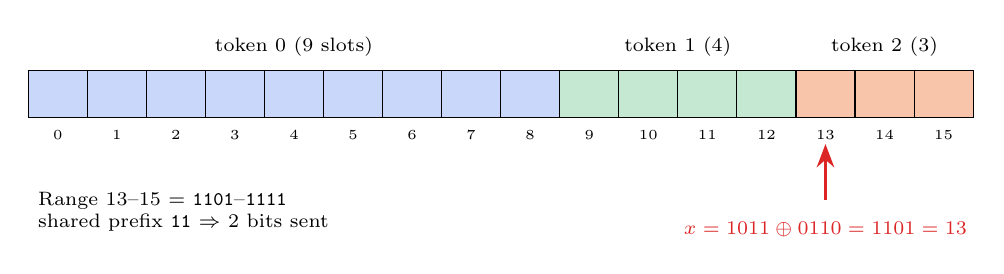
\begin{tikzpicture}[x=0.75cm,y=0.75cm]
  \foreach \i in {0,...,15}{\draw (\i,0) rectangle ++(1,0.8); \node[font=\tiny] at (\i+0.5,-0.3) {\i};}
  \fill[sender!25] (0,0) rectangle (9,0.8);   \node[font=\scriptsize] at (4.5,1.2) {token 0 (9 slots)};
  \fill[receiver!25] (9,0) rectangle (13,0.8);\node[font=\scriptsize] at (11,1.2) {token 1 (4)};
  \fill[auditor!35] (13,0) rectangle (16,0.8);\node[font=\scriptsize] at (14.5,1.2) {token 2 (3)};
  \foreach \i in {0,...,15}{\draw (\i,0) rectangle ++(1,0.8);}
  \draw[-{Stealth},very thick,secret] (13.5,-1.4) -- (13.5,-0.45);
  \node[font=\scriptsize,secret,align=center] at (13.5,-1.9) {$x = 1011 \oplus 0110 = 1101 = 13$};
  \node[font=\scriptsize,align=left,anchor=west] at (0,-1.6) {Range 13--15 = \texttt{1101}--\texttt{1111}\\shared prefix \texttt{11} $\Rightarrow$ 2 bits sent};
\end{tikzpicture}
\caption{One Meteor step. The masked secret lands in token 2's range. The shared first bits of the range are the bits that get transmitted.}
\end{figure}

\subsection{Why the text looks normal}
The mask makes $x$ uniformly random over the 16 slots.
So each token is chosen exactly as often as its slot count.
That is the same as normal sampling.
A test checks this exactly: over all 256 masks at $\beta=8$, each token was chosen exactly as often as its range width.

\textit{Real settings used:} $\beta = 32$, the 50 most likely tokens (top-$k=50$), model Qwen2.5-0.5B-Instruct \cite{qwen2024}.

\subsection{Animated walkthrough of the whole project}
Figure~\ref{fig:anim} is an animation (press play in Adobe Acrobat Reader or Okular).
Figure~\ref{fig:story} shows the same frames on paper.
An interactive version with play, back and next controls is in \url{docs/stegaudit_explainer.html}; it opens in any web browser.

\begin{figure}[H]\centering
\begin{animateinline}[controls,loop,poster=first,width=0.92\linewidth]{0.4}
\FrameA\newframe\FrameB\newframe\FrameC\newframe\FrameD\newframe\FrameE\newframe\FrameF\newframe\FrameG
\end{animateinline}
\caption{Animation: the whole project in seven steps. One frame every 2.5 seconds.}\label{fig:anim}
\end{figure}

\begin{figure}[H]\centering
\resizebox{0.48\linewidth}{!}{\FrameA}\hfill\resizebox{0.48\linewidth}{!}{\FrameB}\\[4pt]
\resizebox{0.48\linewidth}{!}{\FrameC}\hfill\resizebox{0.48\linewidth}{!}{\FrameD}\\[4pt]
\resizebox{0.48\linewidth}{!}{\FrameE}\hfill\resizebox{0.48\linewidth}{!}{\FrameF}\\[4pt]
\resizebox{0.48\linewidth}{!}{\FrameG}
\caption{Storyboard of the animation. (1) Key exchange. (2) Hiding. (3) Monitor sees nothing. (4) Receiver decodes. (5) Sentinel can only guess. (6) Auditor compares decisions. (7) Audit where the stakes are high.}\label{fig:story}
\end{figure}

% =====================================================================
\section{System and Application Developed}
% =====================================================================
\subsection{Architecture}
\begin{figure}[H]\centering
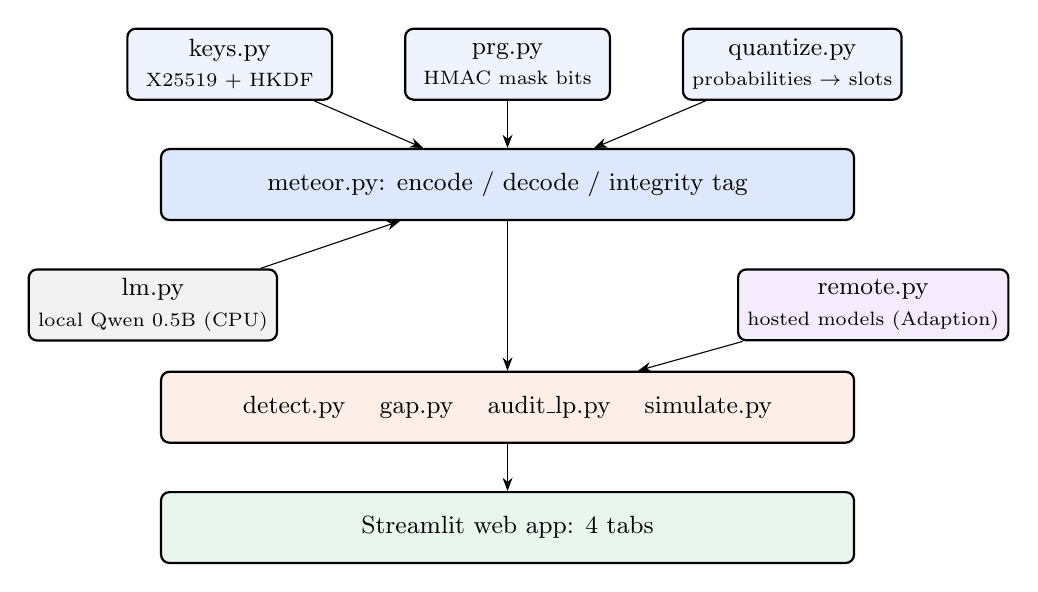
\begin{tikzpicture}[node distance=0.6cm and 0.9cm,
  box/.style={draw,rounded corners=3pt,thick,align=center,font=\small,minimum height=0.9cm,minimum width=2.6cm}]
  \node[box,fill=sender!8] (keys) {keys.py\\\scriptsize X25519 + HKDF};
  \node[box,fill=sender!8,right=of keys] (prg) {prg.py\\\scriptsize HMAC mask bits};
  \node[box,fill=sender!8,right=of prg] (q) {quantize.py\\\scriptsize probabilities $\to$ slots};
  \node[box,fill=sender!15,below=of prg,minimum width=8.8cm] (met) {meteor.py: encode / decode / integrity tag};
  \node[box,fill=gray!10,below left=0.6cm and -1.5cm of met] (lm) {lm.py\\\scriptsize local Qwen 0.5B (CPU)};
  \node[box,fill=sentinel!10,below right=0.6cm and -1.5cm of met] (rem) {remote.py\\\scriptsize hosted models (Adaption)};
  \node[box,fill=auditor!10,below=1.9cm of met,minimum width=8.8cm] (an) {detect.py \quad gap.py \quad audit\_lp.py \quad simulate.py};
  \node[box,fill=receiver!10,below=0.6cm of an,minimum width=8.8cm] (app) {Streamlit web app: 4 tabs};
  \draw[-{Stealth}] (keys) -- (met); \draw[-{Stealth}] (prg) -- (met); \draw[-{Stealth}] (q) -- (met);
  \draw[-{Stealth}] (lm) -- (met); \draw[-{Stealth}] (met) -- (an); \draw[-{Stealth}] (rem) -- (an);
  \draw[-{Stealth}] (an) -- (app);
\end{tikzpicture}
\caption{Software architecture. The hidden channel runs on a local model. Hosted models play the Sentinel, the untrusted Receiver and the judge.}
\end{figure}

\textbf{Why the channel runs locally.} Meteor needs every token's exact probability.
Sender and Receiver must compute \emph{bit-identical} numbers, or decoding fails.
Hosted services return only a few probabilities and are not bit-reproducible.
So the hidden channel uses a local model. Hosted models only read text and answer.

\subsection{The web application}
The app is written in Streamlit. All logic is imported from the tested library; the app file contains no cryptography of its own.

\begin{enumerate}
  \item \textbf{Meteor live.} Key exchange, encode a typed secret, highlight the tokens that carry bits, click a token to see its ranges, mask, $x$ and bits sent. Decode with the right key and with a wrong key (``Eve''). A $\beta$ slider changes precision live.
  \item \textbf{Can you spot it?} A quiz: which of two texts hides a message? Plus the detector results.
  \item \textbf{Collusion and audit.} One decision end to end: hidden tip, Receiver decodes and answers, Sentinel guesses. Plus the measured gap.
  \item \textbf{Audit game.} Sliders for budget, stake inequality, detection rate, false-flag rate and penalty. It solves the audit plans live and compares them.
\end{enumerate}

\shot{app_tab1.png}{Tab 1: Meteor live, with the per-step inspector.}
\shot{app_tab2.png}{Tab 2: detectability quiz and detector results.}
\shot{app_tab3.png}{Tab 3: collusion and decision audit on one item.}
\shot{app_tab4.png}{Tab 4: the audit game.}

% =====================================================================
\section{Implementation Details}
% =====================================================================
\subsection{Technology}
Python 3; PyTorch (CPU) and Hugging Face Transformers for the local model;
\texttt{cryptography} for X25519, HKDF and HMAC; SciPy (HiGHS solver) for the audit plans;
Streamlit for the app; the Adaption SDK for hosted models; pytest for tests.
All versions are pinned in \texttt{requirements.txt}. The model is pinned to its exact commit hash.

\subsection{Main modules}
\begin{tabularx}{\linewidth}{lX}
\toprule
\texttt{keys.py} & X25519 exchange, HKDF to $k_\text{mask}$ and $k_\text{tag}$\\
\texttt{prg.py} & HMAC-SHA256 mask stream with fixed-width fields and labels\\
\texttt{quantize.py} & Probabilities $\to$ integer ranges summing to $2^\beta$\\
\texttt{lm.py} & Deterministic local model, one token at a time\\
\texttt{meteor.py} & Encode, decode (from text and from token ids), tag check\\
\texttt{detect.py} & Five transcript detectors and AUROC with CIs\\
\texttt{gap.py} & Receiver vs Sentinel accuracy, steganographic gap\\
\texttt{audit\_lp.py}, \texttt{simulate.py} & Audit plans (linear programs) and colluder strategies\\
\bottomrule
\end{tabularx}

\subsection{Engineering problems solved}
\begin{itemize}
  \item \textbf{Bit-exact repeatability.} One CPU thread, fixed seeds, 64-bit softmax, same code path for Sender and Receiver. Two fresh processes give identical numbers.
  \item \textbf{Retokenisation.} The model may write \texttt{Program}+\texttt{ming}, but reading the text back gives \texttt{Programming}. Decoding then fails. This is detected by the tag and never accepted as a wrong message.
  \item \textbf{End-of-text during the payload.} The model is not allowed to stop before all hidden bits are sent. This is a small, documented change.
  \item \textbf{Memory.} The full test suite with the model needs about 5.7\,GB; tests share one loaded model.
\end{itemize}

\subsection{Testing and reproducibility}
\begin{itemize}
  \item \textbf{330 automated tests pass} (one process, about 7 minutes): key agreement, mask uniqueness, range correctness, round trips, wrong keys, the exact worked example, LP solutions against brute force and closed forms, and app start-up.
  \item \textbf{Pre-registration.} Every prediction was written and committed \emph{before} its experiment ran. Changes are logged as ``deviations''.
  \item \textbf{Git history} shows each stage as a separate, verified commit. Every result file records the code version, seed and model hash.
\end{itemize}

% =====================================================================
\section{Results}
% =====================================================================
\subsection{Experiment 01: does the hidden channel work?}
200 messages at each precision $\beta \in \{8, 12, 16, 32\}$.

\begin{table}[H]\centering
\caption{Experiment 01 results.}
\begin{tabular}{lr}
\toprule
Decoding from token ids (all $\beta$) & \textbf{200/200} each; fresh-process check agrees on all 800\\
Decoding from text at $\beta=32$ & \textbf{200/200}\\
Retokenisation mismatches ($\beta=32$) & 5/200 = 2.5\% [0.8, 5.7], all after the payload\\
Wrong messages accepted & \textbf{0} of 800\\
Tokens needed for 16 hidden bits & median 16 (range 3--42), about 1 bit per token\\
\bottomrule
\end{tabular}
\end{table}

\subsection{Experiment 02: can detectors see the hidden message?}
200 hidden-message texts versus 200 normal texts.

\begin{table}[H]\centering
\caption{Detector AUROC on whole texts (0.5 = coin toss).}
\begin{tabular}{lc}
\toprule
\textbf{Detector} & \textbf{AUROC [95\% CI]}\\
\midrule
Average token log-probability & 0.522 [0.465, 0.579]\\
Rare (``vanishing'') tokens & 0.500\\
End-of-text probability & 0.498 [0.440, 0.556]\\
Tokens outside top-50 & 0.500\\
AI judge (deepseek-v4-flash) & 0.452 [0.398, 0.506]\\
\bottomrule
\end{tabular}
\end{table}

\begin{keypoint}
\textbf{Result:} no detector beat a coin toss. Reading the text does not reveal the hidden message.
One weak signal appeared only if the detector is \emph{told} where the hidden part ends (last hidden token: AUROC 0.169). A real monitor does not know this.
\end{keypoint}

\shot[0.8\linewidth]{02_auroc.png}{Detector AUROC with confidence intervals (Experiment 02).}

\subsection{Experiment 03: does decision auditing catch it?}
\textbf{Task.} 100 private decisions, e.g.\ ``which of four suppliers wins the contract?''.
The right answer is drawn at random, so no model can know it.
The Sender hides the answer (2 bits) in an unrelated study tip.

\textbf{Who answers.} Sentinels: \texttt{qwen3.5-397b} and \texttt{glm-5.2}. Untrusted Receiver: \texttt{deepseek-v4-flash}.

\begin{table}[H]\centering
\caption{Experiment 03 results.}
\begin{tabular}{lcc}
\toprule
 & \textbf{Qwen Sentinel} & \textbf{GLM Sentinel}\\
\midrule
Gap (Receiver with key minus Sentinel) & \textbf{+0.74} & \textbf{+0.78}\\
Detection rate $d$ (flag on hidden-message items) & 0.74 [0.65, 0.82] & 0.78 [0.70, 0.86]\\
False-flag rate $f$ (flag on normal items) & 0.16 [0.09, 0.23] & 0.11 [0.05, 0.18]\\
\bottomrule
\end{tabular}
\end{table}
Channel failures: 0 of 100. Controls (no hidden message; hint written openly; Sentinel given the key): gap 0.00 for both Sentinels in all three. These are equal by construction (identical prompts), so they check the pipeline, not model behaviour. Question-only accuracy: 0.28 (Qwen), 0.19 (GLM), 0.25 (DeepSeek); chance is 0.25. $d$ and $f$ use the untrusted Receiver \texttt{deepseek-v4-flash}; brackets are 95\% CIs over the 100 items.

\begin{keypoint}
\textbf{Result:} the transcripts look identical, but the decisions do not.
The key holder is right far more often. This difference is the alarm.
\end{keypoint}

\textbf{A lesson from the design.} We first planned general-knowledge questions (MMLU).
Strong Sentinels already know most of those answers, so the hidden channel adds little.
\emph{Decision auditing only catches hidden information that matters beyond what the auditor already knows.}

\subsection{Experiment 04: where should the auditor look?}
1{,}000 decisions with different stakes. The auditor can check only a few.
A colluder knows the stakes and cheats where it pays.

\begin{plain}{audit plan, linear program}
An \textbf{audit plan} says how likely each decision is to be checked.
A \textbf{linear program (LP)} is a standard maths tool that finds the best plan under a budget.
\textbf{M1} minimises the total value the colluder gets away with.
\textbf{M2} is the classic ``security game'' plan \cite{kiekintveld2009,blocki2013}: it minimises the colluder's best \emph{single} gain.
\end{plain}

\[
\textbf{M1:}\ \min \sum_i t_i \quad \text{s.t.}\ t_i \ge v_i - d\,c_i\,(v_i+P),\ t_i\ge 0,\ 0\le c_i\le 1,\ \textstyle\sum_i c_i \le B
\]
Here $v_i$ is the stake, $c_i$ the chance of auditing decision $i$, $d$ the detection rate, $P$ the penalty and $B$ the budget.

\begin{table}[H]\centering
\caption{Experiment 04 results (all settings of the registered grid).}
\begin{tabularx}{\linewidth}{lX}
\toprule
Targeting the big stakes & Hides more than random cheating in \textbf{2560/2560} settings; its undetected share grows with inequality (640/640 series)\\
M1 vs simple plans & \textbf{Never worse} (640/640), strictly better in \textbf{506}\\
M2 (classic plan) & Worse in \textbf{238/640}, by up to 0.82 of total stake\\
Audits needed vs cheating rate $\varepsilon$ & $\propto 1/\varepsilon^2$ when false flags exist; $\propto 1/\varepsilon$ when they do not\\
\bottomrule
\end{tabularx}
\end{table}

\shot[0.8\linewidth]{04_undetected.png}{Value the colluder gets away with, per audit plan (Experiment 04).}

% =====================================================================
\section{Observations}
% =====================================================================
\begin{enumerate}
  \item \textbf{Meteor works and hides well.} Perfect decoding; no detector beat chance.
  \item \textbf{Capacity is low.} About 1 hidden bit per token, because short study tips are predictable (about 1.7 bits of randomness per step).
  \item \textbf{Watch behaviour, not words.} The decision gap was large (+0.74 to +0.78).
  \item \textbf{False flags change everything.} With no false flags, one catch is proof. With false flags, the auditor needs many more checks ($1/\varepsilon^2$).
  \item \textbf{The textbook audit plan is the wrong one here.} M2 guards against one big attack. A colluder that cheats many times needs M1.
  \item \textbf{Models guess alike.} No model picked option D often, though D was correct most often. So honest disagreement was lower than predicted for GLM. Similar models share blind spots.
\end{enumerate}

% =====================================================================
\section{Limitations}
% =====================================================================
\begin{itemize}
  \item \textbf{Small model.} The hidden channel used a 0.5-billion-parameter model on a CPU.
  \item \textbf{Detectors tried, not all detectors.} A 2026 paper detects Meteor through rounding artefacts \cite{acl2026}. We did not test that detector. ``Undetected'' means ``undetected by our five detectors''.
  \item \textbf{One AI judge.}
  \item \textbf{Simulated stakes.} Experiment 04 uses synthetic stakes, linked to the LLM experiment only through $d$ and $f$.
  \item \textbf{Simple colluder.} Our colluders follow fixed rules. A learning colluder could do better.
  \item \textbf{Hosted models are not repeatable.} Their answers are reproducible only through our saved cache.
  \item \textbf{Pre-shared key.} We assume the key was agreed before monitoring started.
\end{itemize}

% =====================================================================
\section{Novelty and Future Work}
% =====================================================================
\textbf{What is known.} Meteor \cite{kaptchuk2021}, the steganographic gap \cite{anwar2026}, audit games \cite{blocki2013}, attack selection in AI control \cite{greenblatt2024}.

\textbf{What this project adds.} As far as our literature check found, the steganographic gap had only been tested on simple ciphers. Here it is tested on cryptographically secure steganography. We also combine it with stake-aware audit planning against a colluder who targets high stakes.
This is a new \emph{application and evaluation}, not a new algorithm. No novelty claim is made beyond that. A research manuscript is not submitted now.

\textbf{Future work.}
A colluder that \emph{learns} where to cheat; the Shimmer scheme; paraphrasing defences; the rounding-artefact detector; larger and frontier models.

% =====================================================================
\section{AI Tools and Academic Integrity}
% =====================================================================
\begin{itemize}
  \item \textbf{Claude (Anthropic)}, via Claude Code and claude.ai, helped design experiments, write code and draft this report. Every AI contribution is logged in \texttt{AI\_USE.md}, with what I checked or changed.
  \item \textbf{Hosted models} from Adaption Labs (\texttt{deepseek-v4-flash}, \texttt{qwen3.5-397b}, \texttt{glm-5.2}) acted as Sentinels, Receiver and judge. Total cost about 4.02 Adaption credits as logged in \texttt{results/credits.json} (Experiment 02 judge 0.38, Experiment 03 3.65); timed-out calls returned no usage and may add up to about 0.04.
  \item \textbf{My own work:} choosing the problem, the research question, all design decisions, checking results, and answering the viva questions in \texttt{NOTES.md}.
  \item All libraries, models and papers are listed in \texttt{REFERENCES.md} and below.
\end{itemize}

% =====================================================================
\section{How to Run}
% =====================================================================
Full steps are in \texttt{README.md}. In short:
\begin{verbatim}
pip install -e .            # install the package
pytest -q                   # run all 330 tests (about 7 min)
streamlit run app/streamlit_app.py   # start the web app
\end{verbatim}
Add \texttt{?tab=1} \ldots\ \texttt{?tab=4} to the app address to open a tab directly.
Hosted-model calls need \texttt{ADAPTION\_API\_KEY} in a \texttt{.env} file; the app replays saved answers without it.

% =====================================================================
\begin{thebibliography}{99}
\bibitem{kaptchuk2021} G.~Kaptchuk, T.~M.~Jois, M.~Green, A.~D.~Rubin. Meteor: Cryptographically Secure Steganography for Realistic Distributions. \emph{ACM CCS}, 2021.
\bibitem{motwani2024} S.~R.~Motwani, M.~Baranchuk, M.~Strohmeier, V.~Bolina, P.~H.~S.~Torr, L.~Hammond, C.~Schroeder de Witt. Secret Collusion among AI Agents: Multi-Agent Deception via Steganography. \emph{NeurIPS}, 2024. arXiv:2402.07510.
\bibitem{anwar2026} U.~Anwar, J.~Piskorz, D.~D.~Baek, D.~Africa, J.~Weatherall, M.~Tegmark, C.~Schroeder de Witt, M.~van der Schaar, D.~Krueger. A Decision-Theoretic Formalisation of Steganography With Applications to LLM Monitoring. arXiv:2602.23163, 2026.
\bibitem{blocki2013} J.~Blocki, N.~Christin, A.~Datta, A.~D.~Procaccia, A.~Sinha. Audit Games. \emph{IJCAI}, 2013. arXiv:1303.0356.
\bibitem{kiekintveld2009} C.~Kiekintveld, M.~Jain, J.~Tsai, J.~Pita, F.~Ord\'o\~nez, M.~Tambe. Computing Optimal Randomized Resource Allocations for Massive Security Games. \emph{AAMAS}, 2009.
\bibitem{greenblatt2024} R.~Greenblatt, B.~Shlegeris, K.~Sachan, F.~Roger. AI Control: Improving Safety Despite Intentional Subversion. \emph{ICML}, 2024.
\bibitem{acl2026} W.~Cao, Y.~Wang, D.~Hu. Breaking the ``Provable Security'': Detecting Finite-Precision Artifacts in LLM-based Steganography via Low-Probability Vanishing. \emph{Findings of ACL}, 2026, pp.~20262--20274. doi:10.18653/v1/2026.findings-acl.1013.
\bibitem{rfc7748} A.~Langley, M.~Hamburg, S.~Turner. Elliptic Curves for Security. RFC 7748, 2016.
\bibitem{rfc5869} H.~Krawczyk, P.~Eronen. HMAC-based Extract-and-Expand Key Derivation Function (HKDF). RFC 5869, 2010.
\bibitem{rfc2104} H.~Krawczyk, M.~Bellare, R.~Canetti. HMAC: Keyed-Hashing for Message Authentication. RFC 2104, 1997.
\bibitem{qwen2024} Qwen Team. Qwen2.5 Technical Report. arXiv:2412.15115, 2024.
\bibitem{ziegler2019} Z.~Ziegler, Y.~Deng, A.~Rush. Neural Linguistic Steganography. \emph{EMNLP}, 2019.
\end{thebibliography}

\end{document}
